% !TeX spellcheck = it_IT
\newpage
\section{Progetto di reti logiche sequenziali}
Le reti logiche sequenziali, avendo una memoria, riassume gli ingressi precedenti in \textbf{stati} del sistema. Questi sono composti da un insieme di bit detto \textbf{variabili di stato}.

\subsection{Macchine a stati finiti}
Le reti sequenziali \textbf{sincrone} possono essere rappresentate tramite \textbf{Finite State Machine}. Una FSM ha $M$ ingressi, $N$ uscite e $k$ bit di stato con $2^k$ possibili stati diversi. Riceve un segnale di \textit{clock} e a volte di \textit{reset}. Si compone di:
\begin{itemize}
	\item Logica di \textbf{stato prossimo} $\sigma$, implementata da reti combinatorie
	\begin{equation*}
		S: \text{IN} \times S \to S
	\end{equation*}
	\item Logica di \textbf{uscita} $\omega$, implementata da reti combinatorie
	\item \textbf{Registro di stato}
\end{itemize}
Le suddividiamo in due tipi:
\begin{itemize}
	\item Macchine di \textbf{Moore}: le uscite dipendono esclusivamente dallo stato attuale della macchina
	\begin{equation*}
		\omega: S \to \text{OUT}
	\end{equation*}
	\item Macchine di \textbf{Mealy}: le uscite dipendono sia dallo stato che dagli ingressi attuali
	\begin{equation*}
		\omega: \text{IN} \times S \to \text{OUT}
	\end{equation*}
\end{itemize}

\subsection{Registri}
\subsubsection{Latch SR}
Il latch SR (set \& reset) permette di memorizzare un bit ed è implementato come segue:
\begin{center}
	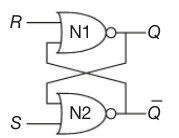
\includegraphics[scale=.4]{latchsr}
\end{center}
L'output non dipende solo dagli input ma anche dallo stato precedente, introducendo un ciclo.
\begin{observation}
	Nel caso in cui sia R che S valgono $1$, la rete non si stabilizza poiché non possiamo eseguire entrambe le operazioni di set e reset contemporaneamente.
\end{observation}

\subsubsection{Latch D}
Per risolvere la problematica del Latch SR, introduciamo un segnale di clock come segue:
\begin{center}
	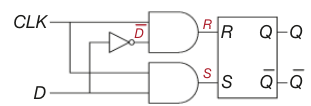
\includegraphics[scale=.4]{latchd}
\end{center}
In questo modo quando il clock vale zero (latch \textbf{opaco}), sia set che reset varranno zero, mentre se vale 1 (latch \textbf{trasparente}) set e reset avranno valori opposti in base all'operazione da fare.
\begin{observation}
	Dato che il clock ha un fronte di salita, il valore $D$ tenderà a stabilizzarsi solo dopo che il clock è alto, causando un ritardo.
\end{observation}

\subsubsection{Flip Flop D}
Per risolvere la problematica del ritardo nel Latch D, implementiamo il Flip Flop D utilizzando due Latch D: \textbf{slave} e \textbf{master}, rispettivamente con il clock non negato e negato.
\begin{center}
	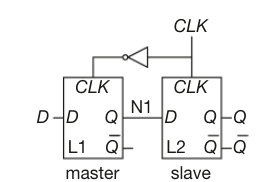
\includegraphics[scale=.4]{flipflopd}
\end{center}
Quando il clock vale $1$ lo slave è aperto alla scrittura e riceve eventuali aggiornamenti dal master per l'output da mostrare che sarà stato scritto su quest'ultimo nel ciclo precedente.\\
Quando il clock vale $0$ il master è aperto alla scrittura mentre lo slave no.\\
Questo permette che la stabilizzazione del clock avvenga solo nel master, rendendo più immediato l'output dallo slave.\\\\
È possibile implementare l'abilitazione alla scrittura tramite un bit \textbf{write enable} messo in AND con il bit del clock.

\subsubsection{Registro}
Il registro si implementa mettendo in parallelo $n$ Flip Flop D.

\subsection{Clock}
Nell'ambito delle prestazioni di reti sequenziali e combinatorie dobbiamo stimare la lunghezza del ciclo di clock, che dipende da:
\begin{itemize}
	\item Ritardi nelle porte logiche
	\item Complessità di $\sigma$
	\item Ritardi di propagazione e contaminazione dei registri
	\item $T_{\text{setup}}$: tempo minimo prima del fronte di salita del clock entro cui i valori degli ingressi devono essere cambiati e stabiliti
	\item $T_{\text{hold}}$: tempo in cui rimangono stabili gli ingressi dopo il fronte di salita del clock affinché il registro riesca a registrare il nuovo valore
	\begin{equation}
		T_{\text{hold}} \leq T_c^{\text{reg}} + T_c^\sigma
	\end{equation}
\end{itemize}

Otteniamo quindi che la stima minima della lunghezza del ciclo di clock è data da:
\begin{equation}
	\tau \geq T_p^{\text{reg}} + \max\{T_p^\omega, T_p^\sigma+T_{\text{setup}}\}
\end{equation}